
%%%%%%%%%%%%%%%%%%%%%%%%%%%%%%%%%%%%%%%%%%%%
\section{Examples of research in Biomedical Engineering}


%%%%%%%%%%%%%%%%%%%%%%%%%%%%%%%%%%%%%%%%%%%%%%%%%%%%%%%%
{
%\paper{}
\begin{frame}{}

\BigSizeFont
How a Biomedical Engineer would help a Sonographer?
\end{frame}
}








%%%%%%%%%%%%%%%%%%%%%%%%%%%%%%%%%%%%%%%%%%%%%%%%%%%%%%%%
{

\paper{Fetal and Mother Numerical Models (FEMONUM) in \url{http://femonum.telecom-paristech.fr}}
%https://perso.telecom-paristech.fr/angelini/projects_research/FEMONUM/femonum_en.html
%https://perso.telecom-paristech.fr/angelini/projects_research/FEMONUM/femonum_en.html

\begin{frame}{Modelling US imaging}
      \begin{figure}
        \centering
        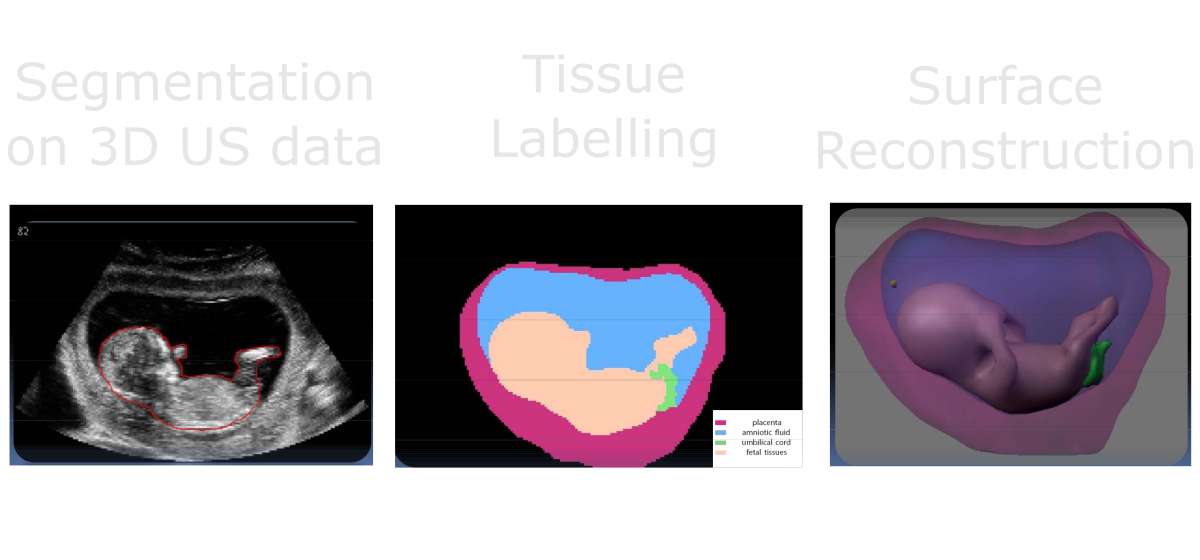
\includegraphics[width=1.0\textwidth]{./figures/modelling-us-imaging/versions/drawing-v02}
        %\caption{}
      \end{figure}
\end{frame}
}




%3D slicer
%* How View Your Baby Ultrasound and Create 3D Printable Model Convert to .stl 3D Slicer for Cura
%https://www.youtube.com/watch?v=WXlwro_n3FM
%
%* View your baby ultrasound and create 3D printable model using free software
%https://www.youtube.com/watch?v=UHq0uyDvhaA
%> A couple of people has shared such data sets publicly on the Slicer forum in this topic:
%https://discourse.slicer.org/t/loading-of-ge-kretz-ultrasound-volumes-vol-file/808/40.
%For example, you can download one of the 3D baby ultrasounds in NRRD format
%(that can be loaded directly into 3D Slicer) from here: https://1drv.ms/u/s!Arm_AFxB9yqHtp93mJQfPqtsVfVeMw
%







%%%%%%%%%%%%%%%%%%%%%%%%%%%%%%%%%%%%%%%%%%%%%%%%%%%%%%%%
{
\paper{Add references}
\begin{frame}
  \frametitle{3D printing a fetus}
  \vspace{10pt}
        \begin{figure}
        \centering
        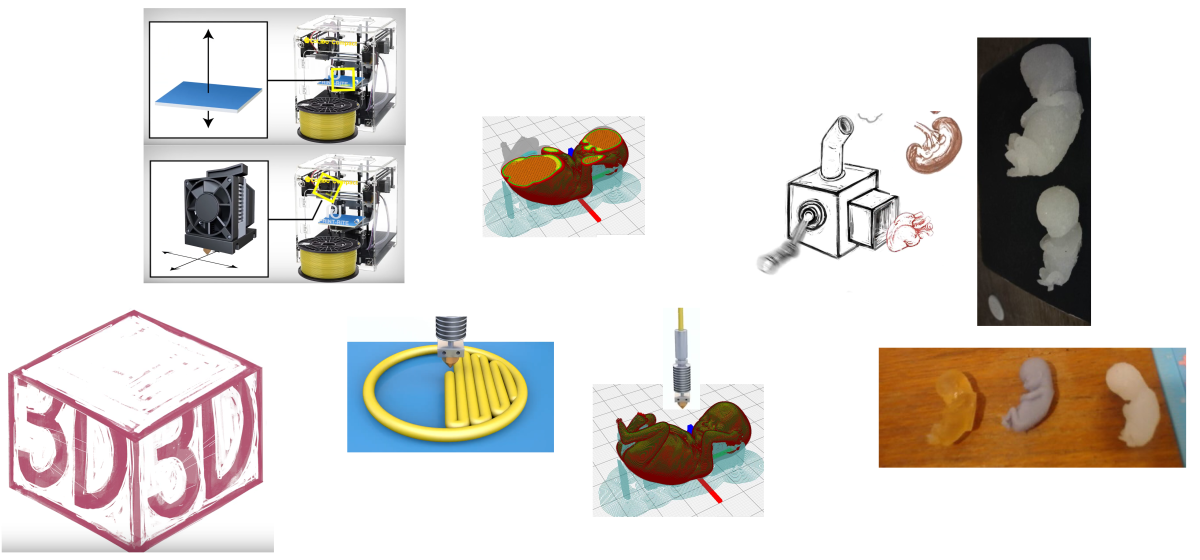
\includegraphics[width=1.0\textwidth]{./figures/3d-printing/why-and-how/versions/drawing-v02.png}
        %\caption{}
      \end{figure}

\end{frame}
}

%%%%%%%%%%%%%%%%%%%%%%%%%%%%%%%%%%%%%%%%%%%%%%%%%%%%%%%%%
%{
%\paper{add references}
%\begin{frame}{Simulator for Ultrasound-Guidance Interventions}
%      \begin{figure}
%        \centering
%        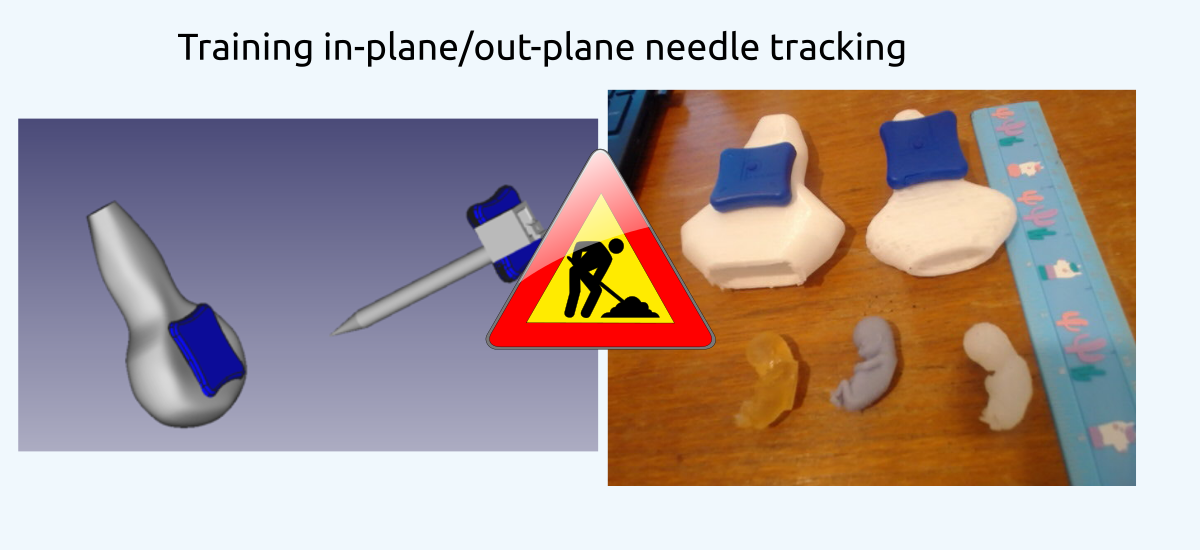
\includegraphics[width=0.9\textwidth]{./figures/sugi/simulator/versions/drawing-v00.png}
%        %\caption{}
%      \end{figure}
%\end{frame}
%}

%%%%%%%%%%%%%%%%%%%%%%%%%%%%%%%%%%%%%%%%%%%%%%%%%%%%%%%%
{
\paper{Add references}
\begin{frame}
  \frametitle{3D printing Fetus}
  \vspace{10pt}
  \begin{center}
    \movie{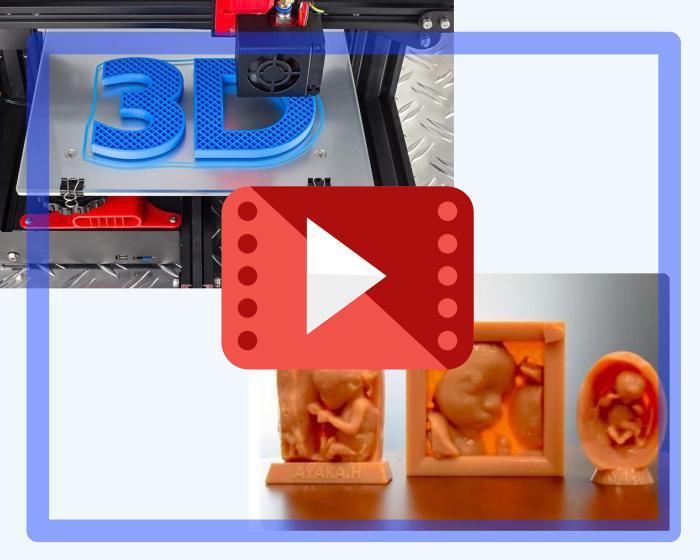
\includegraphics[width=0.5\textwidth]{./figures/3d-printing/video-of-printing-process/versions/drawing-v01.png}}{./figures/3d-printing/video-of-printing-process/videos/apollo17.avi}
  \end{center}
%  \begin{itemize}
%    \item Click on the image to play/pause the video.
%    \item Move pointer to the bottom of the video frame for a draggable position  control.
%  \end{itemize}
\end{frame}
}



%%%%%%%%%%%%%%%%%%%%%%%%%%%%%%%%%%%%%%%%%%%%%%%%%%%%%%%%
{
%\paper{}
\begin{frame}{Interactive DEMO}

\BigSizeFont
Can you identify the face of a fetus with Ultrasound?

\end{frame}
}

%%%%%%%%%%%%%%%%%%%%%%%%%%%%%%%%%%%%%%%%%%%%%%%%%%%%%%%%
{

\paper{3D Slicer in \url{http://slicer.com}}

\begin{frame}{Interactive Ultrasound Imaging}
      \begin{figure}
        \centering
        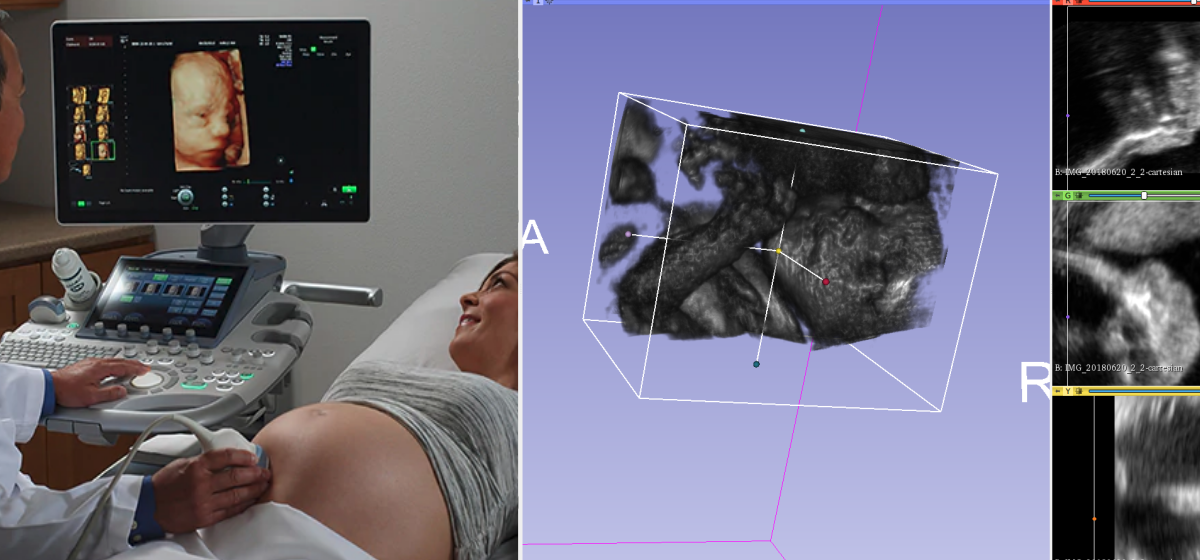
\includegraphics[width=1.0\textwidth]{./figures/3dslicer/versions/drawing-v01.png}
        %\caption{}
      \end{figure}
\end{frame}
}




%%%%%%%%%%%%%%%%%%%%%%%%%%%%%%%%%%%%%%%%%%%%%%%%%%%%%%%%
{
\paper{Wright-Gilbertson M. 2014 in PhD thesis: Xia et al., 2017 in Scientific Reports}
\begin{frame}{Ultrasound Needle-Tracking}
      \begin{figure}
        \centering
        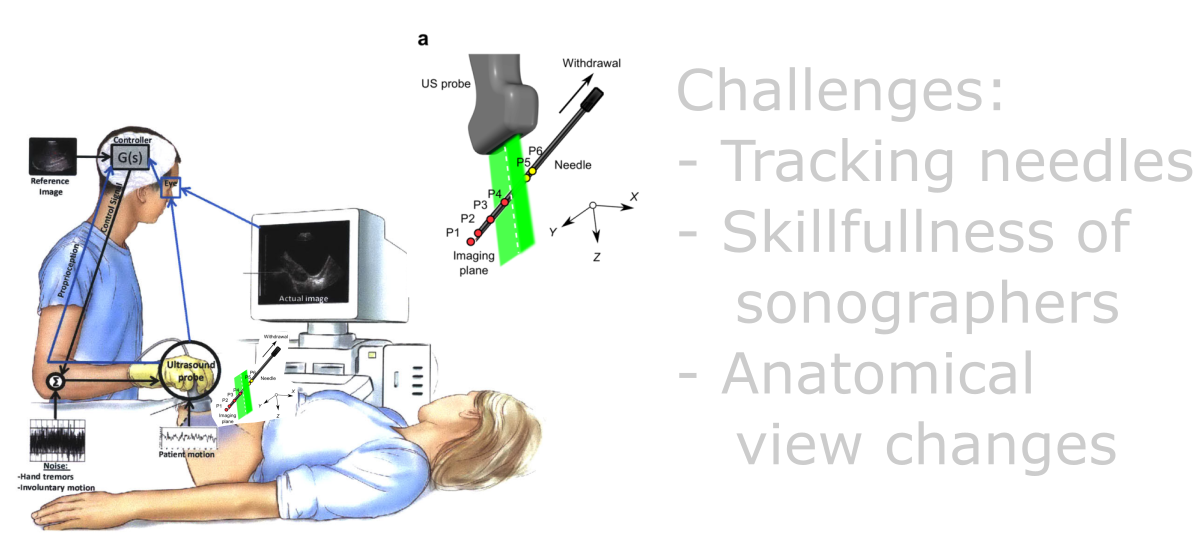
\includegraphics[width=1.0\textwidth]{./figures/sonographer-probe-patient/versions/drawing-v02.png}
        %\caption{}
      \end{figure}
\end{frame}
}







